\documentclass[10pt,a4paper,draft,article]{memoir}
\counterwithout{section}{chapter}

\usepackage[T1]{fontenc}
\usepackage{palatino}
\usepackage{graphicx}
  \graphicspath{{./figs/}}


\usepackage{ifdraft}
\ifdraft{
  \usepackage[final,hyperindex,hyperfootnotes,bookmarksnumbered,colorlinks]{hyperref}
}{
  \usepackage[final,hyperindex,hyperfootnotes,bookmarksnumbered]{hyperref}
}

\usepackage{multirow}
\usepackage{url}
\usepackage[textsize=small]{todonotes}
  %% new command for box about missing references
  \newcommand{\addref}[1][]{\todo[color=red!40,size=\tiny]{Add reference: #1}}

\usepackage{natbib}

\newcommand{\CodingGenesInHistOne}{50}
\newcommand{\PseudoGenesInHistOne}{9}
\newcommand{\TotalGenesInHistOne}{59}

\newcommand{\CodingGenesInHistTwo}{11}
\newcommand{\PseudoGenesInHistTwo}{7}
\newcommand{\TotalGenesInHistTwo}{XXXXX}

\newcommand{\CodingGenesInHistThree}{3}
\newcommand{\PseudoGenesInHistThree}{XXXX}
\newcommand{\TotalGenesInHistThree}{XXXXX}

\newcommand{\CodingGenesInHistFour}{1}
\newcommand{\PseudoGenesInHistFour}{XXXX}
\newcommand{\TotalGenesInHistFour}{XXXXX}

\newcommand{\HistOneSpan}{2.3\,Mbp}
\newcommand{\HistTwoSpan}{105\,kbp}
\newcommand{\HistThreeSpan}{XXXXbp}
\newcommand{\HistFourSpan}{XXXXbp}

\newcommand{\HOneArgLysRatio}{???}
\newcommand{\OthersArgLysRatio}{???}

% 12 coding H2A, 10 coding H3, 6 coding H1
% 15 coding H2B, 12 coding H4
\newcommand{\MarzluffCodingGenesInHistOne}{50}
\newcommand{\MarzluffPseudoGenesInHistOne}{9}
\newcommand{\MarzluffTotalGenesInHistOne}{59}

% 3 coding H2A, 2 pseudo H3, 1 coding H3
% 4 pseudo H2B, 1 coding H2B, 1 coding H4
\newcommand{\MarzluffCodingGenesInHistTwo}{11}
\newcommand{\MarzluffPseudoGenesInHistTwo}{7}
\newcommand{\MarzluffTotalGenesInHistTwo}{XXXXX}

% 1 coding H2A, 1 coding H3
% 1 pseudo H2B, 1 coding H2B
\newcommand{\MarzluffCodingGenesInHistThree}{3}
\newcommand{\MarzluffPseudoGenesInHistThree}{XXXX}
\newcommand{\MarzluffTotalGenesInHistThree}{XXXXX}

% 1 coding H2A
\newcommand{\MarzluffCodingGenesInHistFour}{1}
\newcommand{\MarzluffPseudoGenesInHistFour}{0}
\newcommand{\MarzluffTotalGenesInHistFour}{0}

\newcommand{\MarzluffHistOneSpan}{2.3\,Mbp}
\newcommand{\MarzluffHistTwoSpan}{105\,kbp}
\newcommand{\MarzluffHistThreeSpan}{XXXXbp}
\newcommand{\MarzluffHistFourSpan}{XXXXbp}


\author{David Miguel Susano Pinto and Andrew Flaus}
\title{The canonical core histone catalogue}

\begin{document}
  \maketitle

  \section{Introduction}
    %% Complementary introduction on the chromatin organization and how it's dynamic

    %% short 2-3 lines on chromatin organization and dynamics}
    Histones are among the most abundant proteins in eukaryotic cells and contribute up
    to half the mass of chromatin. They define the structure and accessibility of the
    nucleosome as the fundamental unit of genome organisation. In addition, the reactive
    sidechains of histones are post-translationally modified as a nexus for signalling
    and potentially for heritable epigenetics.

    Histones have been studied for many decades as abundant proteins which were readily
    isolated due to their highly basic chemical character. Successive improvements in
    fractionation revealed 5 main types under a nomenclature as histone H1, H2A, H2B, H3
    and H4\citep{nomenclature}.  %% FIXME should we refer the foreword of the Ciba Foundation symposium 28?
    An additional histone H5 related to H1 is found in nucleus-containing avian
    erythrocytes and has been of research interest due to its elevated binding stability.
    Since the ratio of arginine/lysine is \HOneArgLysRatio\ for H1 and H5 these became known as
    ``lysine-rich'', whereas the remaining 4 histones with ratios \OthersArgLysRatio\ \todo{should
    repeated proteins count twice?} are ``arginine-rich''.
    The demonstration of the nucleosome as the fundamental repeating unit of chromatin revealed
    that H2A, H2B, H3 and H4 associated as an octamer of two copies each within the
    nucleosome core particle, so they are referred to as ``core histones''. H1 and H5
    associate with the linker DNA between nucleosome core particles, and are referred to
    as ``linker histones''.

    Extracting histones from cells and separating them by polyacrylamide gel electrophoresis
    (PAGE) using the strongly anionic detergent sodium dodecyl sulphate (SDS) and neutral
    buffers gives single bands for each histone type. However, PAGE with acetic acid in gels
    containing the non-ionic detergent Triton X--100 and uncharged urea as denaturants
    (TAU or AUT) allows the separation of histones into multiple species due to both
    post-translational modifications and variations in sequence within types.

    There are two recognised classes of histone protein sequence variation as summarised in
    Table~\ref{tab:typical-histone-differences}. ``Variants'' play functionally distinctive
    roles, have lower aggregate abundance,
    and show less identity in alignments. Examples of histone variants are H2A.Z, H2AX, H2Abbd
    and H3.3. Most are significantly expressed outside S~phase of the cell cycle and referred
    to as ``replication independent''~(RI).

    In contrast, ``canonical'' histones contribute to the primary function and bulk nucleosome
    structures. Although the canonical histones are encoded by multiple genes with varying
    sequence, the resulting protein ``isoforms'' differ at only a few sites and are often
    referred to as ``wild type'' sequences. This has led to their portrayal as a single histone
    type, with an implicit suggestion that they can be represented by a single sequence. Because
    a primary role of canonical histones is to package the newly duplicated genome during
    S~phase, they are ``replication dependent''~(RD).

    The two classes of histones are also distinguished by their regulation in humans and other
    metazoans: histone variants typically have unique promoter elements and transcripts that
    are polyadenylated on their 3' termini. \todo{Are they transcribed by pol II?} Canonical
    histones share a common promoter structure (???) and a unique stem-loop in the 3' untranslated
    region that is the basis for regulation of turnover. In general, canonical histone transcripts
    are not thought to be polyadenylated except in \textit{S. cerevisiae}.

    The genes encoding canonical histone isoforms are typically found in clusters in most eukaryotic
    genomes, possibly for regulatory efficiency and to facilitate their sequence conservation. In
    contrast, most variant histones are encoded as single genes outside of the histone clusters.

    \begin{table}
      \centering
      \begin{tabular}{l | l | l | l | l }
        \null     & Expression timing       & Sequence identity & Functional relationships       & Transcript stabilisation \\
        \hline
        Canonical & Replication Dependent   & High              & Isoforms                       & Stem--loop in 3' UTR \\
        Variants  & Replication Independent & Low               & Distinct specialised functions & poly--A tail \\
      \end{tabular}
      \caption{Table 1: General properties of canonical and variant histone proteins.}
      \label{tab:typical-histone-differences}
    \end{table}

    Despite the importance of histones to the organisation of chroamtin, and extensive interest
    in their role in epigenetics and regulation, the curation and classification of human histone
    gene and protein sequences has not been revisited for a decade \cite{Marzluff02}. In this time
    the draft human genome has been finalised and rich annotations have been propogated through gene
    and protein sequence databases. We have exhaustively searched the popular RefSeq and UniProt
    databases to curate and report a number of oversights in untranslated regions, transcripts and
    classification of pseudo genes (Table~\ref{tab:difference-from-Marzluff02}).

    In this paper we provide a comprehensive overview of the nomenclature and distribution of canonical
    and variant histone genes. Furthermore, since curation and annotation are dynamic processes, we have
    implemented an accompanying resource that automatically generates the tables and figures presented
    in the submitted manuscript (Section~\ref{sec:reproducible}) based on the most current data from the NCBI
    RefSeq database.

  \section{Histone genes}

    \subsection{Gene clusters}
      The genes encoding canonical histone isoforms are typically found in clusters in most eukaryotic genomes,
      possibly for regulatory and expression functions and to facilitate sequence conservation. These clusters
      are observed to aggregate within the nucleoplasm with processing factors as Histone Locus Bodies
      (HLBs) similar but distinct from Cajal bodies\addref. In human, there are 4 histone gene clusters which
      are numbered by their size (Table~\ref{tab:histone-gene-count}).

      \subsubsection{Internal cluster organization}
        The major and secondary histone gene clusters,
        HIST1 on chromosome 6, and HIST2 on chromosome 1, contain contiguous high density arrays
        of histone genes. HIST1 encodes \CodingGenesInHistOne{}~functional genes and
        \PseudoGenesInHistOne{}~pseudogenes over a span of \HistOneSpan{} and is the second most
        gene dense region on the megabase scale the genome \addref[Xie 2003]. It is located at the
        distal end of the major histocompatibility complex (MHC) in the extended class~I region at chromosome
        6p21-22 \addref[MHC consortium Nature 1999] which may have an effect on
        its recombination. HIST2 encodes \CodingGenesInHistTwo{}~functional
        genes and \PseudoGenesInHistTwo{}~pseudogenes over a span of \HistTwoSpan{}.
        %%HIST1 spans HIST1H2AA-HIST1H2BO 25726291-27861669; HIST2 spans HIST2H2BF-HIST2H2AB 149754245-149859466 (ensembl genome browser)

        On the other hand, the minor clusters, HIST3 also on chromosome 1, and HIST4 on
        chromosome 12, have only a handful of histone genes, \CodingGenesInHistThree{} and
        \CodingGenesInHistFour{} respectively, interspersed with non-histone coding genes.

        \todo[inline]{Talk about gene density of clusters, GC content, patterns of divergent promoters?}

        In humans, these genes are all jumbled in the clusters unlike
        frogs where the genes appear organized in tandem. Not all genes in the cluster are functional, several have
        been annotated has pseudo-genes, ususally due to not found promotor sequences.

        To note that all H1 genes exist on HIST1 and that HIST4 has a single gene (HIST4H4) which has been reported to be transcripted.

        \missingfigure{diagram of histones organizatin on clusters}



        \subsubsection{Proximity of stability and variation}
        %% Talk about how hyperrecombinational MHC next to HIST1, and deletion-duplication
        %% prone 1q21.1 adjacent to HIST2 (Brunetti-Pierri 2008)

    \subsection{Gene nomenclature}

      Histone genes have a very specific nomenclature that reflects their organization in the genome.

      \begin{figure}
        \centering
%        
\includegraphics[width=\textwidth]{nomenclature-schematic.pdf}
        \caption{Nomenclature}
        \label{fig:nomenclature}
      \end{figure}

      A typical replication histone gene has a name such as HIST1H3B. This name can be split in
      3 parts (Fig.~\ref{fig:nomenclature}): HIST1, H3, and B. The first two parts are self-explanatory,
      an H3 gene on the histone cluster 1. The last letter indicates that is the second H3 gene on the cluster.
      The first gene of the cluster, and by association the start of the cluster, is the gene closest to the telomere
      while the last gene of the cluster, marking the end of the cluster, is the one closer to the centromere. When
      there was only one gene of the histone in a cluster, there was no letter indicating its position. However, there is
      one omission from the list, the gene HIST1H2AE is followed by HIST1H2AG, skipping the letter F. This is due
      to another characteristic of the nomenclature, the names also represent the mouse orthologs which makes it easier
      to cross data between the two animal models. There is a Hist1h2af (capitalization
      of the gene name is different between human and mouse) gene in mouse that simply has no correspondent in human.

      This nomenclature was originally described in \cite{Marzluff02} and made no distinction between
      pseudo and protein coding genes; suspected pseudo genes were still named based on their position
      inside the cluster. ``New'' histone genes have since been found in the clusters,\todo{some of them are just inferred}
      most of them pseudo genes, and others had their type changed from coding to pseudo and
      vice-versa (Table~\ref{tab:difference-from-Marzluff02}).
      This forced some genes to be renamed: HIST2H2AA is now named HIST2H2AA3 (a new H2A coding gene
      HIST2H2AA4 was found between HIST1H2AA and HIST1H2AB);
      and HIST2H2B is now named HIST2H2BA (after the discovery of another H2B coding gene in the
      cluster named HIST2H2BB).\todo{it seems their names are not correspondent to the order in cluster}
      Other new coding genes were discovered at the end of the cluster and as such their names could respect the nomenclature. However,
      several new pseudo genes were discovered in the middle of the cluster. These were named differently, with the suffix PS\#
      and numbered by order of discovery. Genes reported at the time of the nomenclature but had their gene type changed to pseudo
      kept their original names.

      \begin{table}
        \centering
        \begin{tabular}{l | l | l | l }
  Added & Removed & Changed for pseudo & Changed for coding \\
  \hline
  HIST1H2APS1 & HIST2H2AA & HIST2H3C & HIST2H3A \\
  HIST1H2APS2 & HIST2H4 &  &  \\
  HIST1H2APS3 &  &  &  \\
  HIST1H2APS4 &  &  &  \\
  HIST1H2APS5 &  &  &  \\
  HIST2H2AA3 &  &  &  \\
  HIST2H2AA4 &  &  &  \\
  HIST1H2BPS1 &  &  &  \\
  HIST1H2BPS2 &  &  &  \\
  HIST2H2BF &  &  &  \\
  HIST1H3PS1 &  &  &  \\
  HIST2H3D &  &  &  \\
  HIST2H3PS2 &  &  &  \\
  HIST1H4PS1 &  &  &  \\
  HIST2H4A &  &  &  \\
  HIST2H4B &  &  &  \\
\end{tabular}


        \caption{Difference from \cite{Marzluff02}}
        \label{tab:difference-from-Marzluff02}
      \end{table}

      The names for the variants are much more different. With the exception of CENP--A (H3 variant named CENtromeric Protein A),
      all histone variants are named in a similar fashion to H2AFX. The histone type, followed by the letter F (which stands for
      Family). The last characters identify the variant and usually have an historical or functional meaning. For example, H2AFX
      and H2AFZ are named accordingly to their migration order in acetic acid-urea gels.

    \subsection{Gene catalogue}

      \begin{table}
        \centering
%        \begin{tabular}{l | l | l | l | l | l }
  %% what about using HIST# instead of Cluster # on the headers?
  \null & HIST1 & HIST2 & HIST3 & HIST4 & Total \\
  location & 6p21-22 & 1q21 & 1q42 & 12p12 & \null \\
  \hline
  H2A   & 12+5      & 4         & 1         & $-$       & 17+5  \\
  H2B   & 15+2      & 2+4       & 1+1       & $-$       & 18+7  \\
  H3    & 10+1      & 3+3       & 1         & $-$       & 14+4  \\
  H4    & 12+1      & 2         & $-$       & 1         & 15+1  \\
\end{tabular}


        \caption{Count of expected functional histone genes and pseudogenes}
        \label{tab:histone-gene-count}
      \end{table}

      \begin{table}
        \centering
%        \begin{table}
  \centering
  \begin{tabular}{l | l | l | l }
    Gene name & Gene UID & Transcript accession & Protein accession \\
    \hline
     HIST1H2AA & 221613 & NM\_170745 & NP\_734466 \\
     HIST1H2AB & 8335 & NM\_003513 & NP\_003504 \\
     HIST1H2AC & 8334 & NM\_003512 & NP\_003503 \\
     HIST1H2AD & 3013 & NM\_021065 & NP\_066409 \\
     HIST1H2AE & 3012 & NM\_021052 & NP\_066390 \\
     HIST1H2AG & 8969 & NM\_021064 & NP\_066408 \\
     HIST1H2AH & 85235 & NM\_080596 & NP\_542163 \\
     HIST1H2AI & 8329 & NM\_003509 & NP\_003500 \\
     HIST1H2AJ & 8331 & NM\_021066 & NP\_066544 \\
     HIST1H2AK & 8330 & NM\_003510 & NP\_003501 \\
     HIST1H2AL & 8332 & NM\_003511 & NP\_003502 \\
     HIST1H2AM & 8336 & NM\_003514 & NP\_003505 \\
     HIST1H2APS1 $\psi$ & 387319 & N/A & N/A \\
     HIST1H2APS2 $\psi$ & 85303 & N/A & N/A \\
     HIST1H2APS3 $\psi$ & 387323 & N/A & N/A \\
     HIST1H2APS4 $\psi$ & 8333 & N/A & N/A \\
     HIST1H2APS5 $\psi$ & 10341 & N/A & N/A \\
     HIST2H2AA3 & 8337 & NM\_003516 & NP\_003507 \\
     HIST2H2AA4 & 723790 & NM\_001040874 & NP\_001035807 \\
     HIST2H2AB & 317772 & NM\_175065 & NP\_778235 \\
     HIST2H2AC & 8338 & NM\_003517 & NP\_003508 \\
     HIST3H2A & 92815 & NM\_033445 & NP\_254280 \\
  \end{tabular}
  \caption{histone H2A genes reference table}
  \label{tab:h2a-ref}
\end{table}

        \caption{histone H2A genes reference table}
        \label{tab:H2A-ref}
      \end{table}

      \begin{table}
        \centering
%        \begin{tabular}{l | l | l | l }
  Gene name & Gene UID & Transcript accession & Protein accession \\
  \hline
   HIST1H2BA & 255626 & NM\_170610 & NP\_733759 \\
   HIST1H2BB & 3018 & NM\_021062 & NP\_066406 \\
   HIST1H2BC & 8347 & NM\_003526 & NP\_003517 \\
   HIST1H2BD & 3017 & NM\_138720 & NP\_619790 \\
   \null     & \null & NM\_021063 & NP\_066407 \\
   HIST1H2BE & 8344 & NM\_003523 & NP\_003514 \\
   HIST1H2BF & 8343 & NM\_003522 & NP\_003513 \\
   HIST1H2BG & 8339 & NM\_003518 & NP\_003509 \\
   HIST1H2BH & 8345 & NM\_003524 & NP\_003515 \\
   HIST1H2BI & 8346 & NM\_003525 & NP\_003516 \\
   HIST1H2BJ & 8970 & NM\_021058 & NP\_066402 \\
   HIST1H2BK & 85236 & NM\_080593 & NP\_542160 \\
   HIST1H2BL & 8340 & NM\_003519 & NP\_003510 \\
   HIST1H2BM & 8342 & NM\_003521 & NP\_003512 \\
   HIST1H2BN & 8341 & NM\_003520 & NP\_003511 \\
   HIST1H2BO & 8348 & NM\_003527 & NP\_003518 \\
   HIST1H2BPS1 $\psi$ & 100288742 & N/A & N/A \\
   HIST1H2BPS2 $\psi$ & 10340 & N/A & N/A \\
   HIST2H2BA $\psi$ & 337875 & N/A & N/A \\
   HIST2H2BB $\psi$ & 338391 & N/A & N/A \\
   HIST2H2BC $\psi$ & 337873 & N/A & N/A \\
   HIST2H2BD $\psi$ & 337874 & N/A & N/A \\
   HIST2H2BE & 8349 & NM\_003528 & NP\_003519 \\
   HIST2H2BF & 440689 & NM\_001024599 & NP\_001019770 \\
   \null     & \null  & NM\_001161334 & NP\_001154806 \\
   HIST3H2BA $\psi$ & 337872 & N/A & N/A \\
   HIST3H2BB & 128312 & NM\_175055 & NP\_778225 \\
\end{tabular}

        \caption{histone H2B genes reference table}
        \label{tab:H2B-ref}
      \end{table}

      \begin{table}
        \centering
%        \begin{table}
  \centering
  \begin{tabular}{l | l | l | l }
    Gene name & Gene UID & Transcript accession & Protein accession \\
    \hline
     HIST1H3A & 8350 & NM\_003529 & NP\_003520 \\
     HIST1H3B & 8358 & NM\_003537 & NP\_003528 \\
     HIST1H3C & 8352 & NM\_003531 & NP\_003522 \\
     HIST1H3D & 8351 & NM\_003530 & NP\_003521 \\
     HIST1H3E & 8353 & NM\_003532 & NP\_003523 \\
     HIST1H3F & 8968 & NM\_021018 & NP\_066298 \\
     HIST1H3G & 8355 & NM\_003534 & NP\_003525 \\
     HIST1H3H & 8357 & NM\_003536 & NP\_003527 \\
     HIST1H3I & 8354 & NM\_003533 & NP\_003524 \\
     HIST1H3J & 8356 & NM\_003535 & NP\_003526 \\
     HIST1H3PS1 $\psi$ & 387324 & N/A & N/A \\
     HIST2H3A & 333932 & NM\_001005464 & NP\_001005464 \\
     HIST2H3B $\psi$ & 333931 & N/A & N/A \\
     HIST2H3C $\psi$ & 333930 & N/A & N/A \\
     HIST2H3D & 653604 & NM\_001123375 & NP\_001116847 \\
     HIST2H3PS2 $\psi$ & 440686 & N/A & N/A \\
     HIST3H3 & 8290 & NM\_003493 & NP\_003484 \\
  \end{tabular}
  \caption{histone H3 genes reference table}
  \label{tab:h3-ref}
\end{table}

        \caption{histone H3 genes reference table}
        \label{tab:H3-ref}
      \end{table}

      \begin{table}
        \centering
%        \begin{tabular}{l | l | l | l }
  Gene name & Gene UID & Transcript accession & Protein accession \\
  \hline
   HIST1H4A & 8359 & NM\_003538 & NP\_003529 \\
   HIST1H4B & 8366 & NM\_003544 & NP\_003535 \\
   HIST1H4C & 8364 & NM\_003542 & NP\_003533 \\
   HIST1H4D & 8360 & NM\_003539 & NP\_003530 \\
   HIST1H4E & 8367 & NM\_003545 & NP\_003536 \\
   HIST1H4F & 8361 & NM\_003540 & NP\_003531 \\
   HIST1H4G & 8369 & NM\_003547 & NP\_003538 \\
   HIST1H4H & 8365 & NM\_003543 & NP\_003534 \\
   HIST1H4I & 8294 & NM\_003495 & NP\_003486 \\
   HIST1H4J & 8363 & NM\_021968 & NP\_068803 \\
   HIST1H4K & 8362 & NM\_003541 & NP\_003532 \\
   HIST1H4L & 8368 & NM\_003546 & NP\_003537 \\
   HIST1H4PS1 $\psi$ & 10337 & N/A & N/A \\
   HIST2H4A & 8370 & NM\_003548 & NP\_003539 \\
   HIST2H4B & 554313 & NM\_001034077 & NP\_001029249 \\
   HIST4H4 & 121504 & NM\_175054 & NP\_778224 \\
\end{tabular}

        \caption{histone H4 genes reference table}
        \label{tab:H4-ref}
      \end{table}


    \subsection{Gene promoters}

  \section{The transcripts}

    In general, metazoan canonical histones
    are not thought to be polyadenylated, although \textit{S.\ cerevisiae} histone transcript stability
    appears to be regulated by polyadenylation instead of RNA structures.

    \subsection{mRNA expression levels}
      %% levels of mRNA of each histone gene in 2-3 different human cell lines (at least one primary cell line)
      Expression of the RD histone genes is highly regulated by the cell cycle (hence the RD name). Probably due
      to the cell high demand for histone proteins during DNA replication, their expression levels rise dramatically
      during this phase of the cell cycle. During the rest of the cell cycle, histone genes are still transcribed
      but with much lower levels.

      However, there is only a 5-fold increase in their transcription rate at S~phase, compared to the other phases
      of cell cycle so regulation acts strongly at the post-transcriptional level\addref.

      To note however, that each gene seems to have different levels of increased transcription, even between genes in the
      same cluster.

      RI histone genes have expression dependent on their needs (testis specific, DNA damage, etc).

    \subsection{Stem-loop}
      Unlike all the other human genes, RD histone genes lack a poly-A tail for the 3' mRNA processing.
      Instead, they encode a stem-loop followed by a purine-rich Histone Downstream Element (HDE)
      downstream of the stop codon. The stem-loop interacts with the Stem-Loop
      Binding Protein (SLBP) to stabilise the mRNA in S~phase \addref
      while the HDE interacts with U7 snRNA to direct efficient 3 end processing\addref.

      This specific machinery for mRNA processing is a large part of increase on transcription during the S--phase
      since their expression is also regulated by the cell-cycle \addref and allow for the histone mRNA stability \addref.

      Some RD histone genes also have annotated a poly-A tail and in similarlity with H2AFX have two annotated transcripts.
      
      However, RI histone genes do show a poly-A tail with the notable pseudo-exception of H2AFX which has both
      a stem-loop and poly-A tail and transcribes 2 different mRNA (one for each).
  %        \missingfigure{consensus of human stem-loop.}

      No RI histone genes show introns on their genes probably to circumvent the requirement
      for primary transcript processing when histones must be rapidly produced at S--phase.
      However, some of the variants do have introns.

  \section{The proteins}
    %% Consensus for each of them, table with their differences (there's at least 1 error on the Marzulff tables)
    %% table with all gene ids, acession number, official symbols etc
    While some of the histone genes encode the same protein, this is not always the case. On the case of H4 and H3 \todo{are H3 and H4
    maybe more important for the nucleosome structure} the number of unique proteins are low, 3 for H3 and 2 for H4. For H2A and H2B
    this number is much higher.\todo{should I get a table for the number of unique proteins? The more complex table with the mutatinos
    is more complex but says the same}

    The numbering of these proteins amino acids also has a catch. The first methionine is cleaved after expression and as such, it is
    never counter when numbering them.

    \subsection{H2A}
      \begin{figure}
        \centering
%        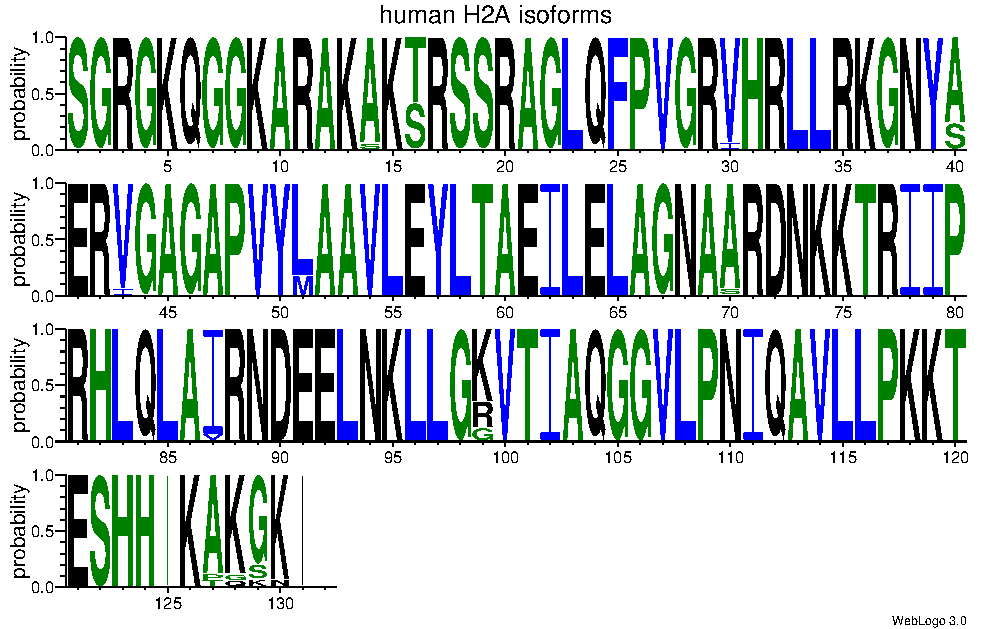
\includegraphics[width=\textwidth]{H2A_weblogo.png}
        \caption{WebLogo of all H2A sequences. The bottom line are the amino acids of H2AFJ whose sequence is different from any of the H2A proteins}
        \label{fig:h2a-weblogo}
      \end{figure}

      \begin{table}
        \centering
%        \missingfigure{consensus and list of changes for each variant --- Marluzz paper style}

        \caption{histone H2A protein consensus}
        \label{tab:H2A-consensus}
      \end{table}

      \todo[inline]{comment on H2AFJ}

    \subsection{H2B}
      \begin{figure}
        \centering
%        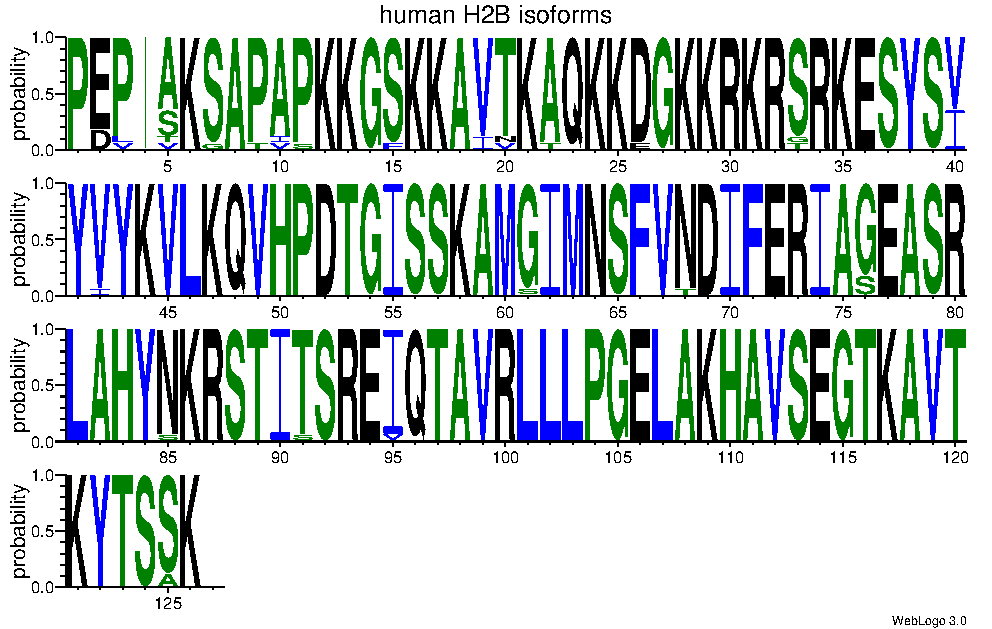
\includegraphics[width=\textwidth]{H2B_weblogo.png}
        \caption{WebLogo of all H2B sequences.}
        \label{fig:h2b-weblogo}
      \end{figure}
      \begin{table}
        \centering
%        \missingfigure{consensus and list of changes for each variant --- Marluzz paper style}

        \caption{histone H2B protein consensus}
        \label{tab:H2B-consensus}
      \end{table}

    \subsection{H3}
      \begin{figure}
        \centering
%        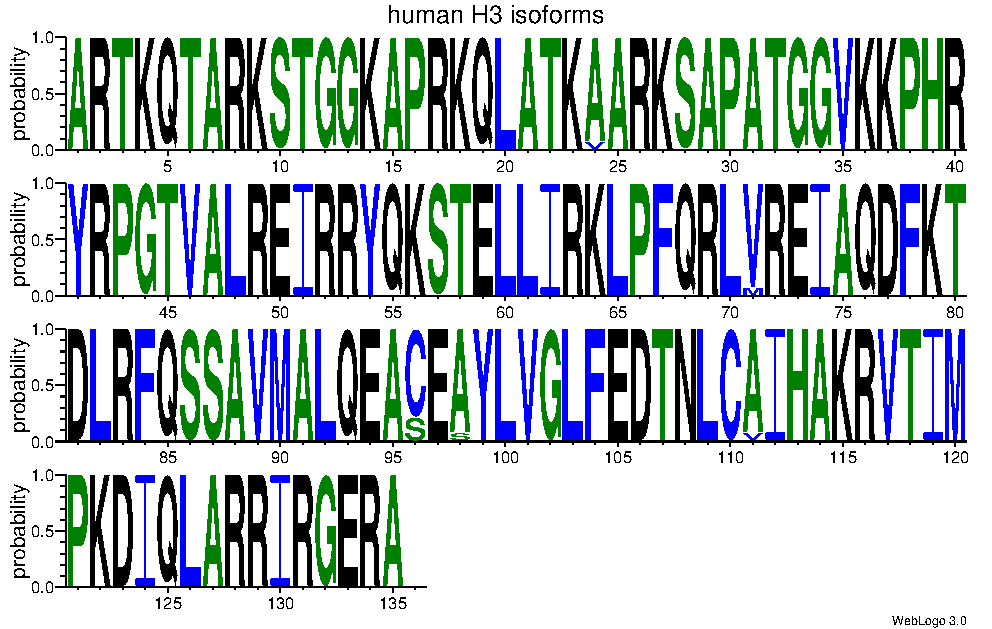
\includegraphics[width=\textwidth]{H3_weblogo.png}
        \caption{WebLogo of all H3 sequences.}
        \label{fig:h3-weblogo}
      \end{figure}
      \begin{table}
        \centering
%        \missingfigure{consensus and list of changes for each variant --- Marluzz paper style}

        \caption{histone H3 protein consensus}
        \label{tab:H3-consensus}
      \end{table}

    \subsection{H4}
      %% these should all be the same bu they are not. And there's an H4 in HIST4
      %% which is also present in mouse, which means has been conserved  in evolution
      With the exception of HIST1H4G, all H4 genes seem to encode the same protein. Even HIST4H4 which is the
      only gene on that ``cluster''.
      \begin{figure}
        \centering
%        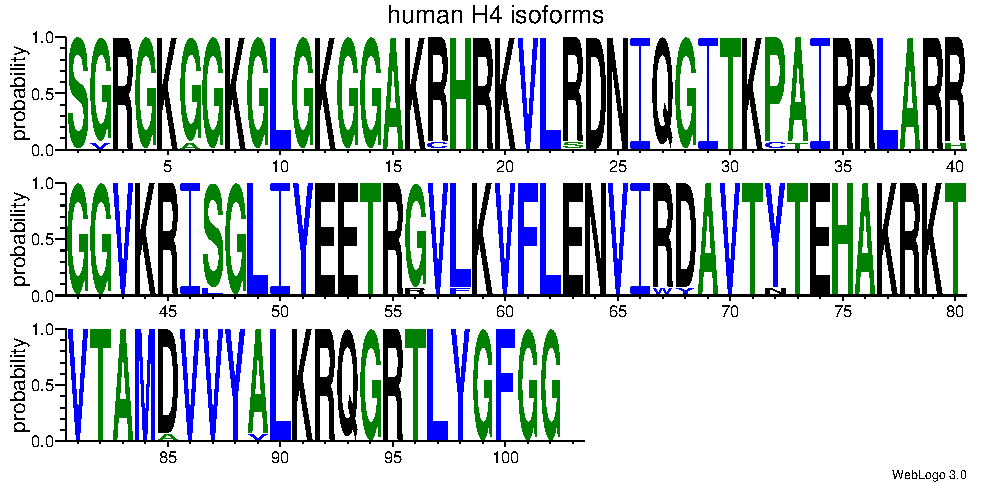
\includegraphics[width=\textwidth]{H4_weblogo.png}
        \caption{WebLogo of all H4 sequences. The non-conserved amino acids are all from one single gene --- HIST1H4G}
        \label{fig:h4-weblogo}
      \end{figure}

      \begin{table}
        \centering
%        \begin{table}
  \centering
  \begin{tabular}{l | l}
    \multicolumn{2}{l}{Human histone H4 consensus (HIST1H4A/B/C/D/E/F/H/I/J/K/L, HIST2H4A/B, HIST4H4)} \\
    \hline
    \multicolumn{2}{l}{svrgkagkg lgkggakchr kvlsdniqgi tkctirrlar hggvkrilgl iyeetrrvfk vflenviwya vtntehakrk tvtamavvyv lkrqgrtl} \\
    \hline
    HIST1H4G   & G2V, G6A, R17C, R23S, P32C, A33T, R40H, S47L, G56R, L58F, R67W, D68Y, Y72N, D85A, A89V \\
  \end{tabular}
  \caption{Count of expected functional histone genes and proteins}
  \label{tab:H4-consensus}
\end{table}

        \caption{Count of expected functional histone genes and proteins}
        \label{tab:H4-consensus}
      \end{table}

  \section{SNP's}
    \todo[inline]{writing is dependent on what is found}

  \section{Canonical isoforms vs.~variants}
    %% Characteristics of a variant are the fact they seem to have special functions. Emphasis
    %% that some canonical may have special functions whicyh no one bothered to check
    %% variants with extra special nomenclature are outside the histone clusters and have poly-A tails (sometimes)
    %% Complain about the lack of information on the different isoforms
    \todo[inline]{Rules and exceptions to definition of canonical and variants. Also point
    that the word canonical suggest antecedence which is not necessarily true (ref to our
    paper and Henikoff's)}

    Variants are the most likely with a standard gene, are considered independent from each other,
    spread around the genome and its expression is mostly independent of cell cycle \todo{explain
    why mostly? Do it next paragraph when complaining the naming}. When people say H2AX that's
    a variant. Note, H2A.2 and H3.2 are not considered variants.

    Both this separation and their naming is very misleading \todo{say that the fact that no one cares is proof?}
    for several reasons.
    \begin{itemize}
      \item The word canonical suggests precedence which is not necessarily true. It has been
            suggested that at least in the case of H2A, the `canonical' gene may have evolved
            from one of the `variant' genes\addref.
      \item Not all `variant' are replication-independent. H2AX gene for example expression
            increases during S--phase together with other `canonical' histones and does show
            a transcript with stem-loop.
      \item The `variant' vs `canonical' separation suggests that there's no variance inside
            the `canonical' which is false. There's several unique protein sequences for each
            `canonical' protein. And even the sometime named H2A.2 and H3.2 variants are actually
            `canonical' histone proteins.
    \end{itemize}

  \section{Sequence extractor}
    To obtain the sequences for the alignment, curation, and IDs for the tables, a perl program using the
    BioPerl modules was written. This program performs a search for genes on entrez, retrieves
    their sequences from the reference assembly, mRNAs and proteins. The sequences are saved in separate files whose
    names are either the gene/transcript/protein name or id.

    The program (bp\_genbank\_ref\_extractor) was released under GPLv3 and is distributed with
    BioPerl since version 1.6.10\todo{actually, it's in the development version, next version might be
    1.7 or 2.0 with the project restructure and everything}.

  \section{Reproducible research}
  \label{sec:reproducible}
    While writing this document, we attempted to follow the principles of reproducible research
    \citep{reproducible-research-bioinformatics, reproducible-research-law}.
    We are also aware of the continuous development of databases and genetic knowledge. As such,
    the source code to replicate the tables and figures shown in this document are freely accessible
    online at \url{https://github.com/af-lab/histone-catalog}. We hope that in the future, it can
    be used to create up to date information
    that reflects the current knowledge on the human histone genes.

    The choice of RefSeq through Entrez over HAVANA through Ensembl was mainly based in one reason --- the ease
    to automate the gene search and retrieve their IDs. Entrez has made available E-utilities with a SOAP interface
    that is already part of the bioperl project. This allowed us to retrieve the search results very easily.
    However, the Ensembl search is done by a Lucene server which is not publicly accessible. Setting up our own
    Lucene instance to provide SOAP services from it was not straightforward for us. The Ensembl perl API is
    also not part of the bioperl project, needing to be installed separately, and is dependent on a very
    out of date version of Bioperl, further complicating its installation. All this would make reproducibility
    of our data a much more difficult process by other researchers.

  \section{Acknowledgements}
    We would like to thank everyone at \#perl and \#bioperl from FreeNode, specially Altreus, mst, LeoNerd and pyrimidine. David Miguel
    Susano Pinto is funded by a personal grant by the Portuguese Foundation for Science and Technology (FCT).

  \bibliographystyle{plainnat}
  \bibliography{references}

\end{document}
